\documentclass[tikz]{standalone}
\usepackage{xcolor}
\newcommand\gry[1]{\definecolor{gry}{RGB}{#1,#1,#1} \def\n{#1}}
\begin{document}
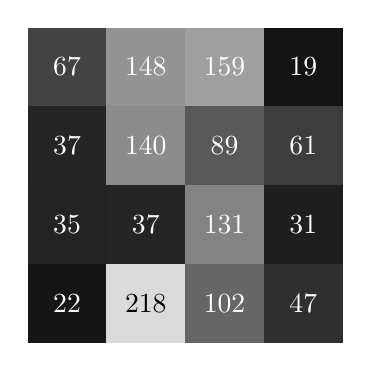
\begin{tikzpicture}
  % row 1
  \gry{67}
  \path[fill=gry] (0,0) rectangle node[color=white]{$\n$} ++(1,-1);
  \gry{148}
  \fill[gry] (1,0) rectangle node[color=white]{$\n$} ++(1,-1);
  \gry{159}
  \fill[gry] (2,0) rectangle node[color=white]{$\n$} ++(1,-1);
  \gry{19}
  \fill[gry] (3,0) rectangle node[color=white]{$\n$} ++(1,-1);
  % row 2: 37   140    89  61
  \gry{37}
  \fill[gry] (0,-1) rectangle node[color=white]{$\n$} ++(1,-1);
  \gry{140}
  \fill[gry] (1,-1) rectangle node[color=white]{$\n$} ++(1,-1);
  \gry{89}
  \fill[gry] (2,-1) rectangle node[color=white]{$\n$} ++(1,-1);
  \gry{61}
  \fill[gry] (3,-1) rectangle node[color=white]{$\n$} ++(1,-1);
  % row 3: 35    37   131  31
  \gry{35}
  \fill[gry] (0,-2) rectangle node[color=white]{$\n$} ++(1,-1);
  \gry{37}
  \fill[gry] (1,-2) rectangle node[color=white]{$\n$} ++(1,-1);
  \gry{131}
  \fill[gry] (2,-2) rectangle node[color=white]{$\n$} ++(1,-1);
  \gry{31}
  \fill[gry] (3,-2) rectangle node[color=white]{$\n$} ++(1,-1);
  % row 4: 22   218   102  47
  \gry{22}
  \fill[gry] (0,-3) rectangle node[color=white]{$\n$} ++(1,-1);
  \gry{218}
  \fill[gry] (1,-3) rectangle node[color=black]{$\n$} ++(1,-1);
  \gry{102}
  \fill[gry] (2,-3) rectangle node[color=white]{$\n$} ++(1,-1);
  \gry{47}
  \fill[gry] (3,-3) rectangle node[color=white]{$\n$} ++(1,-1);
\end{tikzpicture}
\end{document}